\section{Motivating Example}
\label{sec:example}

We next present a real world example to motivate our approach.
Through the example, we demonstrate that developers often ignore the temporal constraints of an API described in the documentation.
We suspect the reason for this phenomena is that the documentation is often verbose and the information is distributed across various pages.
For instance, the PDF version of the documentation for \amazonAPI\footnote{{\small \url{http://awsdocs.s3.amazonaws.com/S3/latest/s3-api.pdf}}} spans 278 pages.
Often developers may not have time (and/or patience) to go through all the documentation and may overlook some temporal constraints of the API,
resulting in defective client applications that invoke API methods in sequences prohibited by documentation. 

\begin{figure}[t]
	\begin{center}
		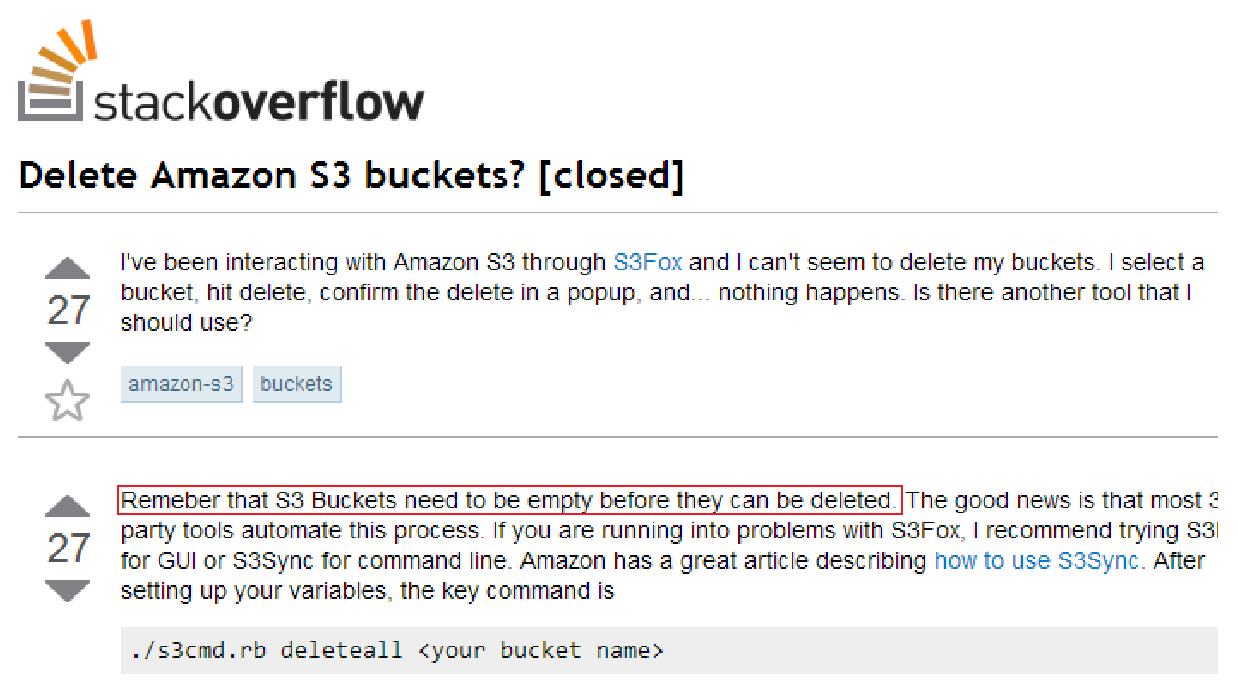
\includegraphics[scale=0.45]{Stackoverflow.eps}
	\end{center}
	\caption{\label{fig:Stackoverflow} The Query posted on Stack Overflow forum regrading Amazon S3 REST API}
\end{figure}

Consider the question asked in \textit{Stack Overflow}~\footnote{{\small \url{http://stackoverflow.com/}}} as shown in Figure~\ref{fig:Stackoverflow}.
Stack Overflow is an online question and answer forum for professional and enthusiast programmers.
The query is about the delete functionality of a third-party software \CodeIn{S3Fox} to interact with \amazonAPI.
The inquisitor complains about an issue in the delete bucket functionality of the \CodeIn{S3Fox}.
The \CodeIn{S3Fox} developers overlooked the constraints in \amazon, causing the issue.
The API document pertaining to the  delete bucket functionality states that before deleting the bucket, the objects in the buckets must be deleted.
\textit{``All objects (including all objects versions and Delete Markers) in the bucket must be deleted before the bucket itself can be deleted''}.
Although the issue was fixed, one of the forum responses contained a recommendation for the inquisitor to switch to another product.
Customer dissatisfaction, such as the one was caused by this issue with the delete bucket functionality, can lead to a loss in revenue.
 
The presented issue can be easily detected using formal analysis tools.
For instance, a specification rule (temporal constraint) can be added to a static checker to verify
the presence of a call to delete object functionality before the call to delete bucket functionality.
%However, existing formal analysis accept only formal specifications but not informal constraints described in natural language.
%Thus, there is need for an approach to automatically translate the constraints described in natural language into a more formal notation.
In next section, we briefly discuss the related work pertinent to our approach.
 








